\documentclass[UTF-8, 12pt]{ctexart}
\setmainfont{Ubuntu}
\setCJKmainfont{STXihei}
\usepackage{fancyhdr}
\usepackage{graphicx}
\title{第十周实验报告}
\author{沈家成}
\date{\today}
\pagestyle{fancy}
\lhead{第十周}
\chead{}
\rhead{\today}
\lfoot{}
\cfoot{\thepage}
\rfoot{}
\renewcommand{\headrulewidth}{0.4pt}
\renewcommand{\headwidth}{\textwidth}
\renewcommand{\footrulewidth}{0pt}

\begin{document}
\maketitle
\section{1367 最大异或}
    \subsection{暴力方法不可取}
    \paragraph{}
    最容易的办法就是一个个遍历,但是那样就是$O(N^2)$的时间复杂度了。很明显,对于两个30000的数列,这种方法是不可取的。

    \subsection{怎么样可以取到最大值}
    \paragraph{}
    异或运算的真值表如下:
    \begin{equation}
        \begin{array}{ccc}
            A & B & A\ xor\ B \\
            0 & 0 & 0 \\
            0 & 1 & 1 \\
            1 & 0 & 1 \\
            1 & 1 & 0
        \end{array}
    \end{equation}
    \paragraph{}
    所以,异或运算可以理解为不进位的加法。因此,想要得到最大值,就是需要参加运算的两个数,各数位上的尽量不同,尤其是高位的,如:
    \begin{equation}
        \begin{array}{cccccccc}
            0 & 0 & 0 & 1 & 1 & 0 & 1 & 1 \\
            1 & 1 & 1 & 0 & 0 & 1 & 0 & 0 \\
            1 & 1 & 1 & 1 & 1 & 1 & 1 & 1
        \end{array}
    \end{equation}
    \paragraph{}
    因此,可以考虑将前一个数列组织成一个便于计算异或的结构,再用第二个数列中的元素遍历,从而得到最大值。考虑到这些数字都可以表达为32位二进制数,每位都是0或1,因此可以用树的结构。
    \paragraph{}
    比如,第一个数列的元素为:
    \begin{equation}
        \begin{array}{cccc}
            1 & 1 & 1 & 0 \\
            1 & 0 & 1 & 0 \\
            1 & 0 & 0 & 1 \\
            0 & 1 & 0 & 1 \\
            0 & 0 & 1 & 1 \\
            0 & 0 & 1 & 0
        \end{array}
    \end{equation}
    \paragraph{}
    就可以构造如下的树。根结点留空,左右孩子分别表示最高位的0和1。左右孩子再各自分开,这样只需要四层就可以表示所有的四位二进制数了。
    \centering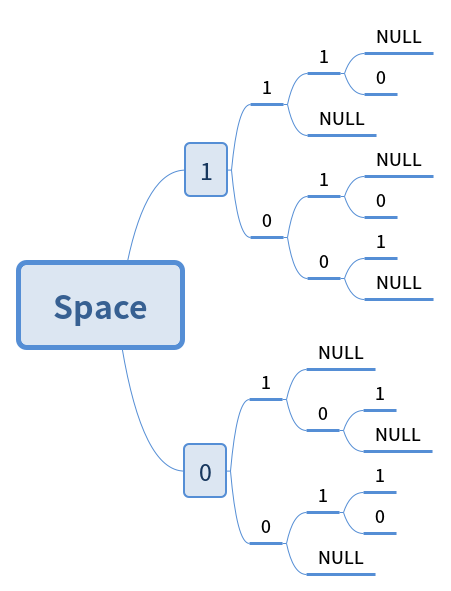
\includegraphics[width = .7\textwidth]{Tree.png}\\
    \paragraph{}
    \paragraph{}
    之后,对于第二个数列中的每个元素,只需要根据这棵数,自高到低,每次选择最好的方案,尽量01配对,就可以得到最大值了。

	    
\section{1219 重要的逆序数列}
	\subsection{普通逆序对}
    \paragraph{}
    用暴力枚举法,会达到$O(N^2)$的时间复杂度,时间性能不够好。用查找树,虽然可以在$O(logN)$的时间内查找插入,但是无法得知查找数字的顺序,也就无法计算逆序。
    \paragraph{}
    为了找到可行的办法,可以先从简单的情况考虑。如果数列的前半部分和后半部分是排好序的,是否会有容易的办法呢?
      \[1, 2, 3, 7, 5, 6, 8 ,9 \]
    \paragraph{}
    此时,可以将前半部分和后半部分看做两个数组。问题就转化为两个有序数组的归并过程要多少步。
    \[A_i: 1, 2, 3, 7 \] 
    \[B_i: 5, 6, 8 ,9 \]
    \paragraph{}
    首先,比较两个数列的首元素,第一个数列的较小,符合小的在前面,没有逆序对产生,放入暂存区。
    \[A_i: 2, 3, 7 \]
    \[B_i: 5, 6, 8 ,9 \]
    \[X_i: 1\]
    重复,直到第二个数列的首元素较小。
    \[A_i: 7 \]
    \[B_i: 5, 6, 8 ,9 \]
    \[X_i: 1, 2, 3\]
    在第一个数列中查找5的位置,共有1个元素(7)比它大,因此产生了一个逆序数。
    \[A_i: 7 \]
    \[B_i: 6, 8 ,9 \]
    \[X_i: 1, 2, 3, 5(+1)\]
    依然是第二个数列的首元素8较大,在第一个数列中,有1个元素(7)比它大,因此产生了一个逆序数。
    \[A_i: 7 \]
    \[B_i: 8 ,9 \]
    \[X_i: 1, 2, 3, 5(+1), 6(+1)\]
    第一个数列的元素较小,放入暂存区。第一个元素已经归并,用第二个数列续尾,完成归并。
    \[A_i: null \]
    \[B_i: 8 ,9 \]
    \[X_i: 1, 2, 3, 5(+1), 6(+1), 7\]
    \subsection{重要的逆序数}
    \paragraph{}
    重要的逆序数,区别在于只有大于两倍才能判定为逆序数。因此,只要在第二个数列元素大于第一个数列时,查找两倍的数列二元素位置,即可。

\section{1550 留下的水}
    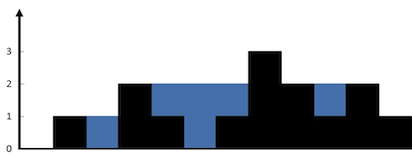
\includegraphics[width = .8\textwidth]{Water.png}
    \subsection{纵向看法}
    \paragraph{}
    纵向就是从左往右看。
    \paragraph{}
    第一个位置高度为0,不可能有水,跳过,下一个。
    \paragraph{}
    第二个位置高度为1,有可能有水,究竟有没有要看之后的情况。
    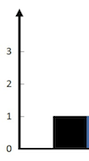
\includegraphics[width = .2\textwidth]{Water_1.png}
    \paragraph{}
    第三个位置高度为1,结合前一个位置高度为1,这个地方是可能有水的,而且最多一个单位。\\
    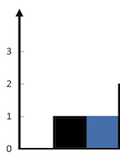
\includegraphics[width = .2\textwidth]{Water_2.png}
    \paragraph{}
    这样寻找下去,程序就很复杂了。所以这不是一个好的角度。

    \subsection{横向看法}
    \paragraph{}
    正难则反,如果横向来看,思路就简单了很多。
    \paragraph{}
    第一层,最左和最右都是实心的地面,中间应该都是水,但是被实心的地面占据了,所以水的体积就是中间的空间减去占据的空间。\\
    \paragraph{}
    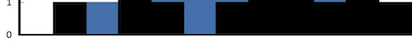
\includegraphics[width = .9\textwidth]{Water_3.png}
    \paragraph{}
    第二层,同样的,中间的空间减去占据的空间就是水的空间。而且,和第一层完全没有关系,代码结构就很清晰明了。
    \paragraph{}
    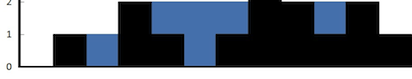
\includegraphics[width = .9\textwidth]{Water_4.png}
\end{document}
